
\chapter{Database management}

\section{Save configuration}

Pressing "Save Configuration to Database" opens a dialog box where you can enter the
name of the new custom configuration:

\begin{figure}[H]
\centering
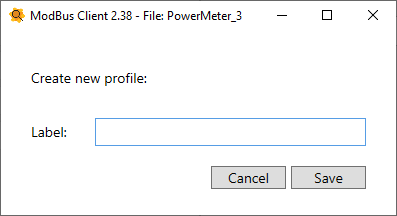
\includegraphics[width=0.35\textwidth]{../Img/SaveProfile.PNG}
\caption{Save new profile}
\end{figure}

Pressing "Save" inside the "Json" folder creates a folder with the name inserted.
DO NOT overwrite existing folders, to make changes to a custom configuration
simply open it. The changes will be saved automatically when closing
of the main window (eventually the user can save the current state from the "File"->"Save menu"
or with the shortcut "Ctrl + S").

\section{Configuration path}

The "Json" folder contains a directory for each profile. The
"Default" folder contains the program configuration when no
custom configurations is selected (if you use the program without loading a specific 
profile, any
change is saved in this folder). The other folders are generated when you save the
current configuration as a new profile.

\begin{figure}[H]
\centering
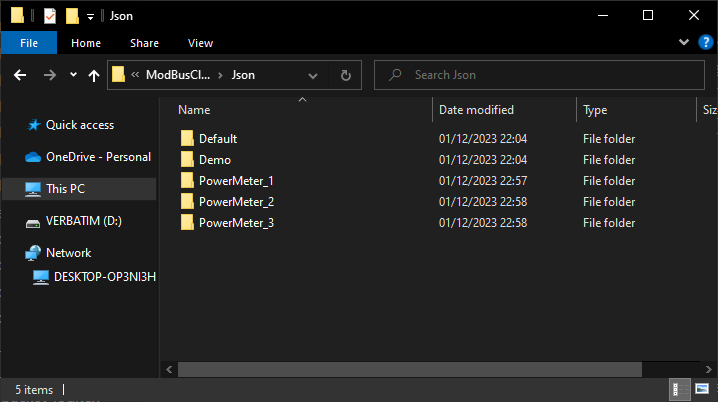
\includegraphics[width=0.45\textwidth]{../Img/DatabaseDirectory.PNG}
\caption{Database profile directory}
\end{figure}

The user in normal use does not need to make changes directly in this folder, 
simply use the forms to save and load profiles directly from the main window.

\newpage
\section{Load configuration}

Pressing "Load configuration from Database" allows you to load a configuration
previously saved:

\begin{figure}[H]
\centering
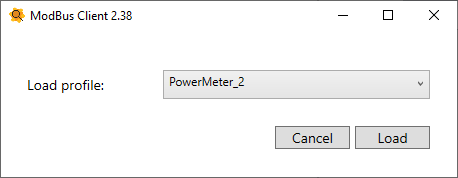
\includegraphics[width=0.45\textwidth]{../Img/LoadProfile.PNG}
\caption{Load profile}
\end{figure}

Once a custom configuration is loaded any changes entered into the program
will be saved in the custom folder without changing the structure of the configuration
"Default".

To import or export a custom Profile use the "Manage database" tool,
here you can export a profile as a .zip file, import a profile 
exported from another client or simply select the profile to be loaded.
When you close the window, automatically the selected profile is loaded into the client.

\begin{figure}[H]
\centering
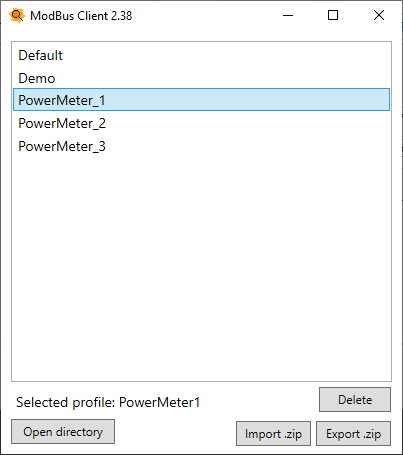
\includegraphics[width=0.40\textwidth]{../Img/DatabaseManager.PNG}
\caption{Database manager}
\end{figure}

Starting with version v2.37, profiles can be uploaded 
directly in the home tab via the drop-down menu provided:

\begin{figure}[H]
\centering
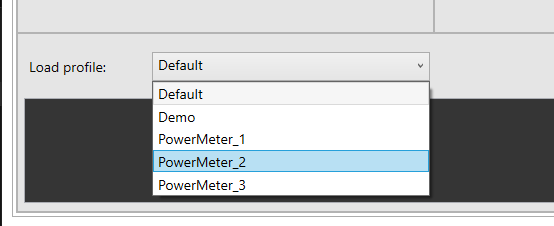
\includegraphics[width=0.50\textwidth]{../Img/ProfileHome.PNG}
\caption{Homepage profile selection}
\end{figure}